\chapter{Experiment}\label{sec:twod_setup}
%
		\begin{figure}[b!]
			\centering
			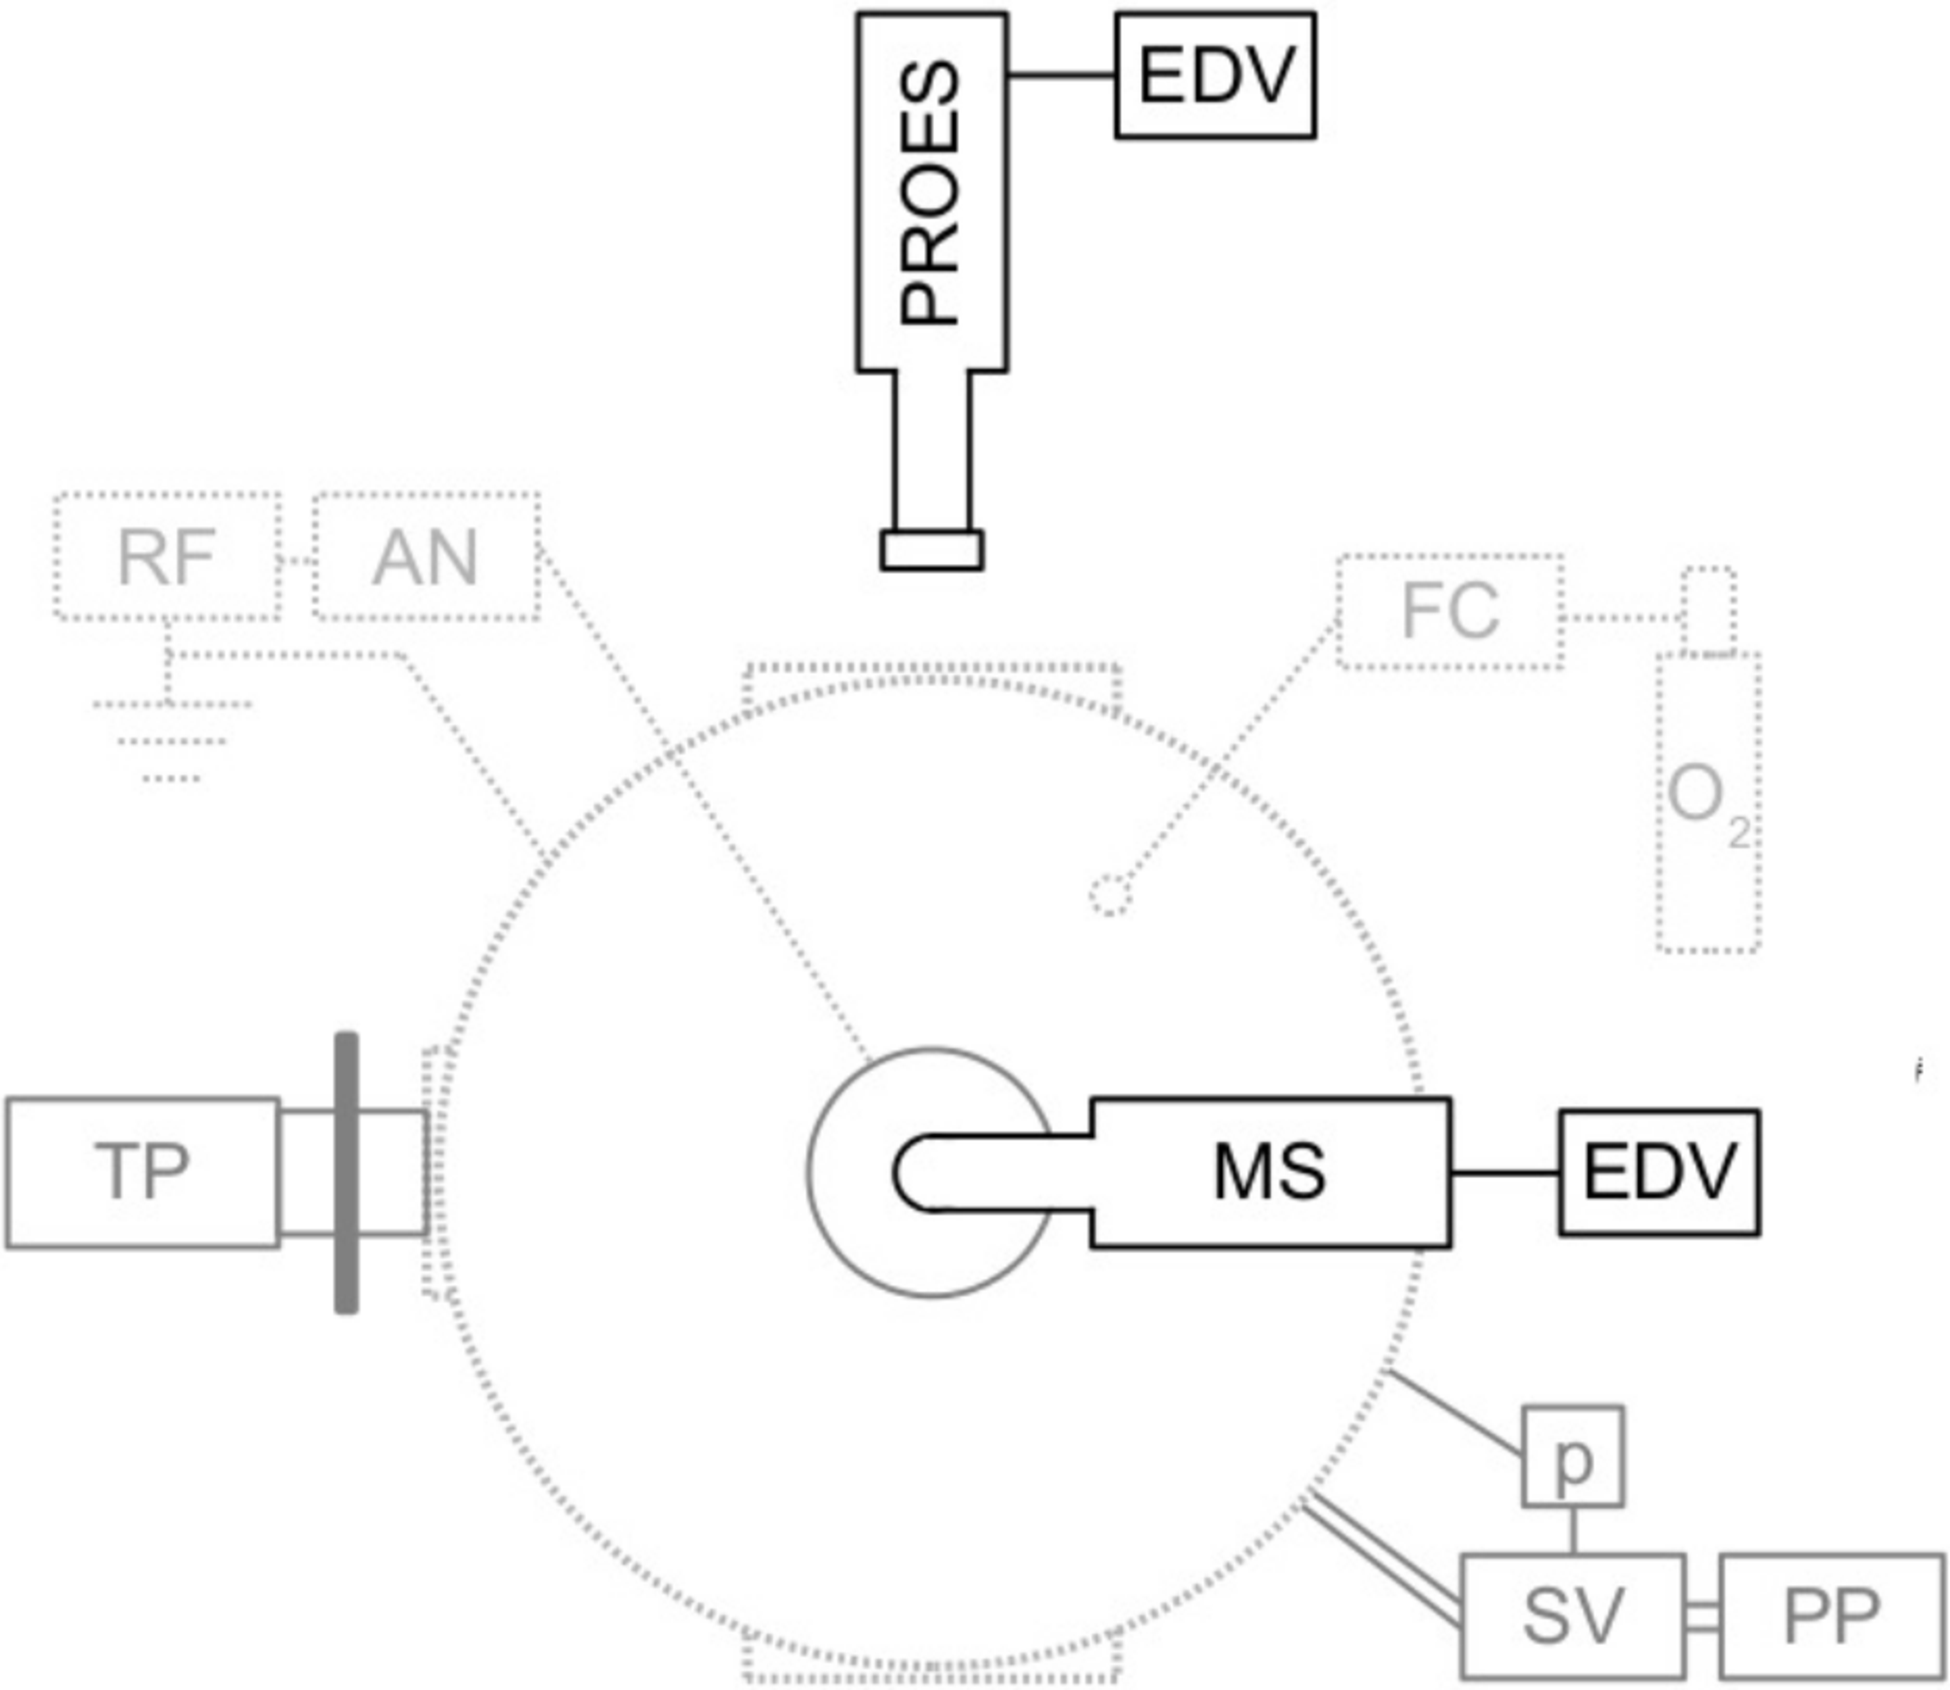
\includegraphics[width=0.7\textwidth]{figures/chamber_exp.pdf}
			\caption[Experiment schematic of cylindrical symmetric ccrf discharge]{%
				Top-down view schematic of the experiment~\cite{Scheuer15},~\cite{Kullig12}. Shown is the setup %
				without microwave interferometer, like it was used by Küllig et al.}\label{fig:discharge_chamber}
		\end{figure}
%		
		\begin{figure}[!t]
			\centering
    		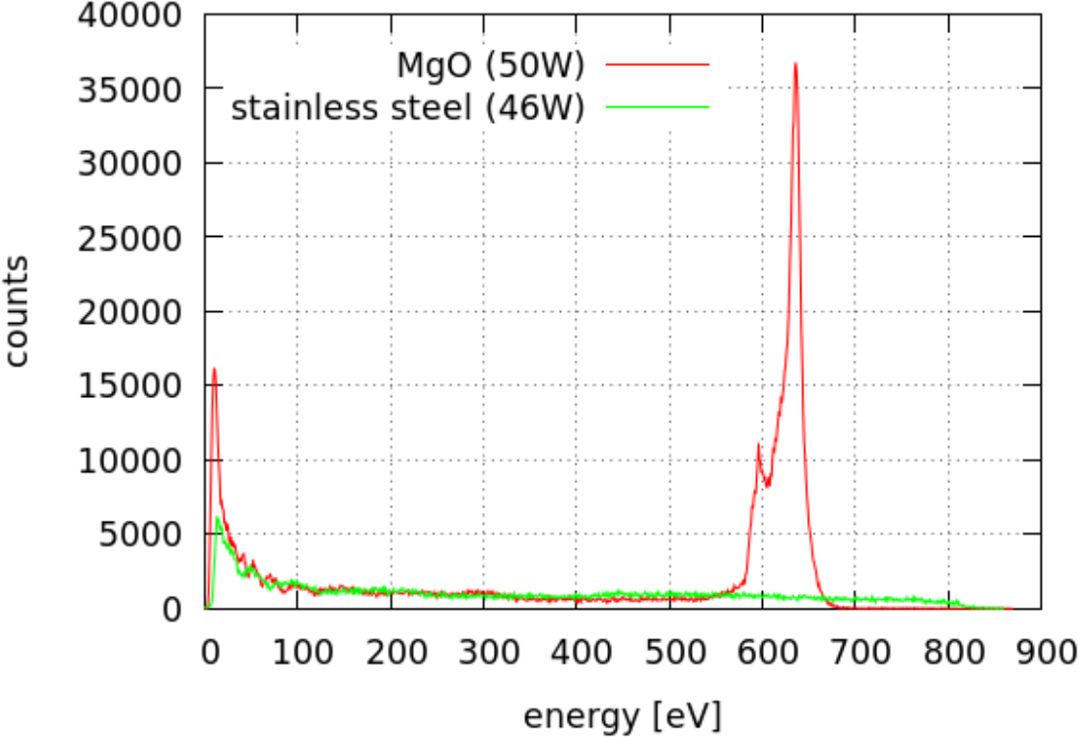
\includegraphics[width=0.8\textwidth]{figures/niondist_material.png}
            \caption[Experimental negative and positive ion EDF for differen materials]{%
                Positive and negative ion energy distribution %
                functions at different cathode power outputs and %
                materials.~\cite{Scheuer15}}
        \label{fig:expresults}
    \end{figure}
%        
		The experiment by Scheuer et al.~\cite{Scheuer15} is used for this study. It consists of a cylindrical stainless steel vacuum chamber, filled with oxygen at low pressures and gas flow rates (see~\autoref{fig:discharge_chamber}). It has a diameter and height of $\unit[40]{cm}$ respectively and was filled with the process gas oxygen (O$\ix{2}$) at $\unit[5]{sccm}$ (\fett{FC}). The discharge configuration consists of an electrode in the centre with $\unit[10]{cm}$ of diameter and a rf generator, constantly operating at a frequency of $\unit[13,56]{MHz}$ and power outputs between $5$ and $\unit[150]{W}$ (\fett{RF} and \fett{AN}), leading to applied voltages in the range of $100$--$\unit[1500]{V}$. The electrode gap was about \SI{5}{\centi\metre}. Shielding and discharge enclosure/chamber walls are grounded. This results in a large area ratio between grounded and driven electrode producing an asymmetric plasma. The powered electrode was coupled capacitively with the external generator. The self bias voltage $U\ix{sb}$ ranged, depending on power output and discharge pressure, from $-100$ up to $\unit[500]{V}$. In~\cite{Kullig12} the experiment was pulsed with short discharges at a frequency of $\unit[10]{Hz}$. Line integrated measurements of average electron density gave  $\tenpo{11}$--$\unit[\tenpo{12}]{cm^{-3}}$. Showing a schematic top-down view of the experiment is~\autoref{fig:discharge_chamber}. Here, the large ratio between driven and grounded parts is easily recognised.\\
		The figure includes further diagnostics like a mass spectrometer (\fett{MS}) and phase resolved optical emission spectroscopy (\fett{PROES}). The latter measured the densities via line integration across the plasma volume. The MS is a key instrument for the investigation pursued in this thesis, as it also measures particle numbers energy resolved. For example, the ions created via secondary processes in the discharge sheath are accelerated towards the bulk and thus get into the MS with their characteristic speeds and mass. A significant increase of electron density was found for rf powers larger than $\unit[50]{W}$ or $\unit[-220]{V}$ self bias voltage~\cite{Kullig12}. This led to a correlating negative oxygen ion density reduction and decrease of the electronegativity ratio $n_{i,-}/n\ix{e}$ from 4 to 0.03. During a different operation mode --- called $\alpha$-mode, contrary to the afore-mentioned $\gamma$-mode --- at less than $\SI{50}{\watt}$ output power, electronegativity rises again, as well as the electron temperature $T\ix{e}$, yielding higher rate coefficients for, e.g.\@ dissociative electron attachment and the alike.\\
	    Experimental results of positive and negative ion distribution function measured by the mass spectrometer are shown in~\autoref{fig:expresults}. The numbers of $O^{-}$ detected on the anode is much lower than those of $O^{+}\ix{2}$. Both distribution functions show a low energy peak and a following plateau up to several hundred $\unit{eV}$. For the positive ion EDF there is a peak at around \SIrange{15}{20}{\electronvolt}, depending on the material and input power. For $MgO$ only we can find a large number of high energy, namely \SIrange{600}{700}{\electronvolt}, negative ions at the anode. 
%
    \begin{figure}[!h]
        \centering
        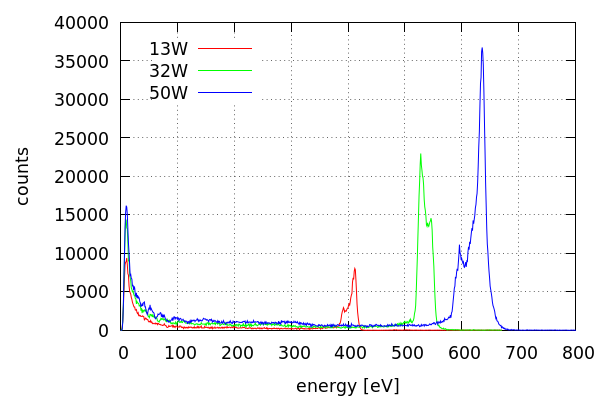
\includegraphics[width=0.8\textwidth]{figures/SFB/neg_mg.png}
        \caption[EDF of negative ions for different discharge powers]{%
            Energy distribution of negative ions $O^-$. Experimental %
            results for $MgO$ measured at the anode for different rf powers.}
        \label{fig:expresults_power}
    \end{figure}
